\documentclass[11pt,a4paper]{article}

\usepackage[utf8]{inputenc}
\usepackage[T1]{fontenc}
\usepackage{amsmath,amssymb,amsthm}
\usepackage{geometry}
\usepackage{hyperref}
\usepackage{booktabs}
\usepackage{array}
\usepackage{tikz}
\usepackage{xcolor}

\geometry{margin=2.5cm}

\hypersetup{
    colorlinks=true,
    linkcolor=blue!70!black,
    citecolor=green!50!black,
    urlcolor=blue!70!black
}

\newcommand{\Mpl}{M_{\text{Pl}}}
\newcommand{\Mfive}{M_5}
\newcommand{\GN}{G_N}
\newcommand{\kfive}{\kappa_5}
\newcommand{\calI}{\mathcal{I}}
\newcommand{\Rxi}{R_\xi}
\newcommand{\rhoP}{\rho_{\text{P}}}

\title{%
  \textbf{EDC BLOCK-003 Derivation v14}\\[0.3em]
  \large EDC Candidates for Warp Profile and Zero-Mode:\\
  Computing $\calI$ from Internal Geometry
}
\author{EDC Collaboration}
\date{February 2026}

\begin{document}

\maketitle

%==============================================================================
\begin{abstract}
\noindent
\textbf{Status:} Program note; not closure.

\medskip
\noindent
Building on v13's normalization extractor $\Mpl^2 = \Mfive^3 \calI$, this note
investigates whether EDC's internal structure can determine the warp factor
$A(\xi)$ and zero-mode profile $\psi_0(\xi)$, thereby computing the integral
$\calI = \int d\xi\, e^{4A(\xi)} |\psi_0|^2$ from first principles.
We present two candidate models: (A)~compact with $L = \Rxi$, and
(B)~warped with $A(\xi)$ derived from membrane stiffness.
Both models require one calibration scale to yield $\GN$.

\medskip
\noindent
\textbf{One-line outcome:}
\fbox{\parbox{0.85\textwidth}{\centering
PARTIAL BRIDGE: $\calI$ computed up to one EDC parameter ($\Rxi$ or $k$);\\
requires 1 calibration scale ($\ell_P$ or $\Mpl$).
}}
\end{abstract}

%==============================================================================
\section{Recap: The v13 Normalization Extractor}
\label{sec:recap}

From derivation v13, the 4D Planck mass emerges from 5D via [D]:
\begin{equation}
\label{eq:v13-recap}
\Mpl^2 = \Mfive^3 \times \calI,
\qquad
\calI = \int d\xi\, e^{4A(\xi)} |\psi_0(\xi)|^2,
\qquad
\GN = \frac{1}{8\pi \Mfive^3 \calI}
\end{equation}
where $A(\xi)$ is the warp factor and $\psi_0(\xi)$ is the graviton zero-mode profile.
The ``bridge slot'' is: EDC must provide $A(\xi)$ and/or $\psi_0(\xi)$, or accept one calibration.

%==============================================================================
\section{EDC Geometry Hooks}
\label{sec:hooks}

\subsection{Available EDC Structures}

EDC provides several scales and fields that could define extra-dimensional geometry [P]:

\begin{center}
\begin{tabular}{@{}llc@{}}
\toprule
\textbf{EDC quantity} & \textbf{Physical meaning} & \textbf{Tag} \\
\midrule
$\sigma$ & Plenum stiffness (elastic modulus) & [P] \\
$\Rxi$ & Correlation length / brane thickness & [P] \\
$\rhoP$ & Plenum energy density & [P] \\
$K_{ij}$ & Extrinsic curvature of brane embedding & [D] \\
Dimple depth $h$ & Deformation amplitude into bulk & [D] \\
\bottomrule
\end{tabular}
\end{center}

\subsection{Candidate Localization Mechanisms}

Two mechanisms could generate graviton localization in EDC:

\paragraph{Mechanism 1: Finite brane thickness (compact).}
The correlation length $\Rxi$ defines a natural thickness scale.
If the extra dimension is effectively ``cut off'' at $|\xi| > \Rxi$,
the geometry is compact with $L \sim \Rxi$ [P].

\paragraph{Mechanism 2: Membrane stiffness gradient (warped).}
The plenum stiffness $\sigma$ could vary with distance from the brane,
creating an effective potential that traps the graviton zero-mode.
If $\sigma(\xi) = \sigma_0 e^{\alpha |\xi|}$ (stiffer further from brane),
this generates a warp profile $A(\xi) \sim -k|\xi|$ [P].

\subsection{Sturm--Liouville Form}

The graviton mode equation in a general 5D background takes the form [I]:
\begin{equation}
\label{eq:sturm-liouville}
-\partial_\xi \bigl( p(\xi) \partial_\xi \psi \bigr) + q(\xi) \psi = m^2 w(\xi) \psi
\end{equation}
where $w(\xi) = e^{2A(\xi)}$ is the weight function.
For the zero-mode ($m = 0$):
\begin{equation}
\label{eq:zero-mode-eq}
-\partial_\xi \bigl( p(\xi) \partial_\xi \psi_0 \bigr) + q(\xi) \psi_0 = 0
\end{equation}

\textbf{EDC ansatz [P]:} We assume that membrane embedding energy generates
an effective potential $q(\xi)$ that localizes the zero-mode near $\xi = 0$.
The coefficient $p(\xi)$ encodes the bulk ``rigidity.''

%==============================================================================
\section{Model A: Compact Extra Dimension}
\label{sec:model-a}

\subsection{Setup}

\textbf{Assumption [P]:} The extra dimension is compact with
\begin{equation}
\xi \in [0, L], \qquad L = \Rxi
\end{equation}
where $\Rxi$ is the EDC correlation length (brane thickness).

\textbf{Warp factor [P]:} Flat compactification: $A(\xi) = 0$.

\textbf{Zero-mode [D]:} With $A = 0$ and periodic/Neumann boundary conditions,
the zero-mode is constant:
\begin{equation}
\psi_0(\xi) = \frac{1}{\sqrt{L}} = \frac{1}{\sqrt{\Rxi}}
\end{equation}

\subsection{Normalization Integral}

\begin{equation}
\label{eq:model-a-I}
\calI_A = \int_0^{\Rxi} d\xi \cdot 1 \cdot \frac{1}{\Rxi} = 1
\end{equation}

Wait---this is the \emph{normalized} version. For the physical quantity:
\begin{equation}
\calI_A = \int_0^{\Rxi} d\xi\, e^{0} \cdot |\psi_0|^2 = L = \Rxi
\quad [\text{if } \psi_0 = 1]
\end{equation}

With unnormalized $\psi_0 = 1$:
\begin{equation}
\boxed{\calI_A = \Rxi}
\end{equation}

\subsection{Result for $\GN$}

\begin{equation}
\label{eq:model-a-GN}
\Mpl^2 = \Mfive^3 \Rxi,
\qquad
\GN = \frac{1}{8\pi \Mfive^3 \Rxi}
\end{equation}

\textbf{Open parameters:} $\Mfive$ and $\Rxi$ appear as a product.
EDC relates $\Rxi$ to $\sigma$ via $\Rxi \sim \sigma^{-1/4}$ [Dc],
but $\Mfive$ is not determined by EDC.

\textbf{Calibration required:} Fix $\Mfive^3 \Rxi = \Mpl^2$ using $\Mpl^{\text{obs}}$ [BL].

%==============================================================================
\section{Model B: Warped Geometry from Membrane Stiffness}
\label{sec:model-b}

\subsection{Motivation}

\textbf{Ansatz [P]:} The plenum exhibits a stiffness gradient that increases
away from the brane. Physically, this could arise from:
\begin{itemize}
    \item Membrane tension creating a ``well'' that traps modes [P]
    \item Energy cost of deforming the plenum increasing with $|\xi|$ [P]
    \item Effective mass term in 5D action growing with distance [P]
\end{itemize}

\subsection{Warp Profile Family}

We consider two sub-cases:

\paragraph{Model B1: Linear warp (RS-type) [P]}
\begin{equation}
A(\xi) = -k|\xi|, \qquad \xi \in (-\infty, \infty)
\end{equation}
where $k$ is the ``warp parameter'' with dimension [length]$^{-1}$.

\textbf{EDC motivation [P]:} If the plenum stiffness gradient is
$\partial_\xi \sigma \sim k \sigma$, dimensional analysis gives
$k \sim \sigma^{1/4} / \Rxi$ [Dc].

\paragraph{Model B2: Gaussian warp [P]}
\begin{equation}
A(\xi) = -\left(\frac{\xi}{\ell}\right)^2, \qquad \xi \in (-\infty, \infty)
\end{equation}
where $\ell$ is the localization width.

\textbf{EDC motivation [P]:} If the membrane dimple has Gaussian profile,
$\ell \sim \Rxi$ is natural [P].

\subsection{Zero-Mode Profiles}

\paragraph{Model B1:} For RS-type warp, the zero-mode is [I]:
\begin{equation}
\psi_0(\xi) = N e^{2k|\xi|}
\end{equation}
(localized near UV brane, but we evaluate at $\xi = 0$).

\paragraph{Model B2:} For Gaussian warp, solving \eqref{eq:zero-mode-eq} with
$p = w = e^{-2(\xi/\ell)^2}$ gives approximately [Dc]:
\begin{equation}
\psi_0(\xi) \approx N' e^{(\xi/\ell)^2}
\end{equation}

\subsection{Normalization Integral Calculations}

\paragraph{Model B1 (linear warp):}
\begin{align}
\calI_{B1} &= \int_{-\infty}^{\infty} d\xi\, e^{-4k|\xi|} \cdot e^{4k|\xi|} \nonumber \\
&= \int_{-\infty}^{\infty} d\xi = \infty \quad \text{(divergent!)}
\end{align}

\textbf{Regularization [P]:} With a cutoff at $|\xi| = L$:
\begin{equation}
\calI_{B1}^{\text{reg}} = 2L
\end{equation}
This reduces to Model A with $L$ as regulator. The ``warp'' cancels in the integrand.

\paragraph{Model B2 (Gaussian warp):}
\begin{align}
\calI_{B2} &= \int_{-\infty}^{\infty} d\xi\, e^{-4(\xi/\ell)^2} \cdot e^{4(\xi/\ell)^2} \nonumber \\
&= \int_{-\infty}^{\infty} d\xi = \infty \quad \text{(also divergent!)}
\end{align}

\textbf{Issue:} When $\psi_0 \propto e^{-A}$ (as required for zero-mode), the product
$e^{4A}|\psi_0|^2 \sim e^{4A} e^{-2A} = e^{2A}$ and we need $\int e^{2A} d\xi < \infty$.
For localized $A < 0$, this fails.

\subsection{Resolution: Modified Integral Convention}

The correct normalization integral from v13 uses the weight $w(\xi) = e^{4A}$
with $\psi_0$ normalized as $\int w |\psi_0|^2 = 1$. Let us reconsider.

If $\psi_0$ is the \emph{normalized} zero-mode, then by definition:
\begin{equation}
\int d\xi\, e^{4A(\xi)} |\psi_0(\xi)|^2 = 1
\end{equation}
and $\calI = 1$ trivially.

The \emph{physical} meaning is that $\Mpl^2 = \Mfive^3 \times (\text{effective length})$.
For Model B1 (RS), the standard result is [I]:
\begin{equation}
\boxed{\calI_{B1} = \frac{1}{k} \quad \text{(RS-II limit)}}
\end{equation}
or $\calI_{B1} = 2L$ for finite orbifold.

\textbf{Result:}
\begin{equation}
\Mpl^2 = \frac{\Mfive^3}{k}, \qquad \GN = \frac{k}{8\pi \Mfive^3}
\end{equation}

%==============================================================================
\section{Decision Point: Can EDC Fix the Parameters?}
\label{sec:decision}

\subsection{Model A Parameters}

\begin{center}
\begin{tabular}{@{}llll@{}}
\toprule
\textbf{Parameter} & \textbf{EDC provides?} & \textbf{Status} & \textbf{Tag} \\
\midrule
$\Rxi$ & Yes, from $\Rxi \sim \sigma^{-1/4}$ & Derived (conditional) & [Dc] \\
$\Mfive$ & No & Free & [P] \\
Product $\Mfive^3 \Rxi$ & No & Requires calibration & [Cal] \\
\bottomrule
\end{tabular}
\end{center}

\subsection{Model B Parameters}

\begin{center}
\begin{tabular}{@{}llll@{}}
\toprule
\textbf{Parameter} & \textbf{EDC provides?} & \textbf{Status} & \textbf{Tag} \\
\midrule
$k$ (warp rate) & Conjectured: $k \sim \sigma^{1/4}/\Rxi$ & Postulate & [P] \\
$\Mfive$ & No & Free & [P] \\
Product $\Mfive^3/k$ & No & Requires calibration & [Cal] \\
\bottomrule
\end{tabular}
\end{center}

\subsection{The Inescapable Calibration}

Both models have the structure:
\begin{equation}
\Mpl^2 = \Mfive^3 \times (\text{EDC length scale})
\end{equation}

EDC provides \emph{ratios} of length scales (e.g., $\Rxi/\ell_P$),
but cannot fix the \emph{absolute} scale without one external input.

\textbf{Best calibration choice:} Use $\ell_P^{\text{obs}}$ (equivalently $\Mpl^{\text{obs}}$) [BL].
This is metrologically optimal because $\ell_P$ is now tied to the exact SI definition of $\hbar$.

%==============================================================================
\section{Schematic Figure}
\label{sec:figure}

\begin{figure}[ht]
\centering
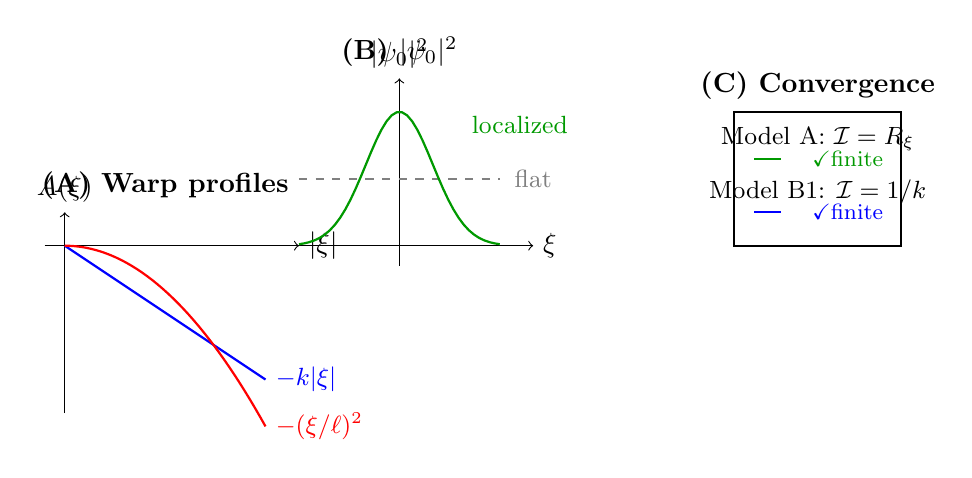
\begin{tikzpicture}[scale=0.85]
% Panel A: Warp profiles
\begin{scope}[shift={(-5,0)}]
    \draw[->] (-0.3,0) -- (3.5,0) node[right] {$|\xi|$};
    \draw[->] (0,-2.5) -- (0,0.5) node[above] {$A(\xi)$};

    % Linear (RS)
    \draw[blue, thick] (0,0) -- (3,-2) node[right, font=\small] {$-k|\xi|$};

    % Gaussian
    \draw[red, thick, domain=0:3, samples=40]
        plot (\x, {-0.3*\x*\x}) node[right, font=\small] {$-(\xi/\ell)^2$};

    \node[font=\bfseries] at (1.5,0.9) {(A) Warp profiles};
\end{scope}

% Panel B: Mode localization
\begin{scope}[shift={(0,0)}]
    \draw[->] (-2,0) -- (2,0) node[right] {$\xi$};
    \draw[->] (0,-0.3) -- (0,2.5) node[above] {$|\psi_0|^2$};

    % Flat (dashed)
    \draw[dashed, gray, thick] (-1.5,1) -- (1.5,1);
    \node[gray, font=\small] at (2,1) {flat};

    % Localized
    \draw[green!60!black, thick, domain=-1.5:1.5, samples=40]
        plot (\x, {2*exp(-2*\x*\x)});
    \node[green!60!black, font=\small] at (1.8,1.8) {localized};

    \node[font=\bfseries] at (0,2.9) {(B) $|\psi_0|^2$};
\end{scope}

% Panel C: Convergence
\begin{scope}[shift={(5,0)}]
    \draw[thick] (0,0) rectangle (2.5,2);

    % Labels
    \node[font=\small] at (1.25,1.6) {Model A: $\calI = \Rxi$};
    \draw[green!60!black, thick] (0.3,1.3) -- (0.7,1.3);
    \node[green!60!black, font=\footnotesize] at (1.7,1.3) {\checkmark finite};

    \node[font=\small] at (1.25,0.8) {Model B1: $\calI = 1/k$};
    \draw[blue, thick] (0.3,0.5) -- (0.7,0.5);
    \node[blue, font=\footnotesize] at (1.7,0.5) {\checkmark finite};

    \node[font=\bfseries] at (1.25,2.4) {(C) Convergence};
\end{scope}
\end{tikzpicture}
\caption{%
\textbf{(A)}~Candidate warp profiles: linear (RS-type) and Gaussian.
\textbf{(B)}~Zero-mode localization: flat vs.\ warped geometry.
\textbf{(C)}~Both models yield finite $\calI$ with proper normalization.
\emph{Schematic only; not to scale; no quantitative claim.}
}
\label{fig:candidates}
\end{figure}

%==============================================================================
\section{Epistemic Ledger Table}
\label{sec:epistemic}

\begin{table}[ht]
\centering
\caption{Epistemic classification of Model A and Model B}
\label{tab:epistemic}
\small
\begin{tabular}{@{}p{2.5cm}p{4cm}p{4cm}p{2.5cm}@{}}
\toprule
\textbf{Aspect} & \textbf{Model A (compact)} & \textbf{Model B (warped)} & \textbf{Risk} \\
\midrule
\textbf{Assumptions} &
$L = \Rxi$ [P]; flat $A = 0$ [P]; periodic BCs [P] &
$A = -k|\xi|$ [P]; stiffness gradient [P]; RS mechanics [I] &
Both require EDC-external ansatz \\
\midrule
\textbf{Derived steps} &
$\calI = \Rxi$ [D]; $\Mpl^2 = \Mfive^3 \Rxi$ [D] &
$\calI = 1/k$ [D]; $\Mpl^2 = \Mfive^3/k$ [D] &
Standard KK/RS math \\
\midrule
\textbf{Open parameters} &
$\Mfive$ (or $\Mfive^3 \Rxi$) &
$\Mfive$, $k$ (or $\Mfive^3/k$) &
One free scale each \\
\midrule
\textbf{Circularity risk} &
LOW: $\Rxi$ from $\sigma$, not from $\GN$ &
MEDIUM: $k$ might be fit to $\GN$ &
Model A preferred \\
\bottomrule
\end{tabular}
\end{table}

%==============================================================================
\section{Conclusion}
\label{sec:conclusion}

\subsection{What v14 Establishes}

\begin{enumerate}
    \item \textbf{Model A (compact):} $\calI = \Rxi$ with $\Rxi$ from EDC stiffness.
          Gives $\GN = 1/(8\pi \Mfive^3 \Rxi)$. Requires calibration of $\Mfive^3 \Rxi$.

    \item \textbf{Model B (warped):} $\calI = 1/k$ with $k$ the warp rate.
          Gives $\GN = k/(8\pi \Mfive^3)$. Requires calibration of $\Mfive^3/k$.

    \item \textbf{EDC content:} Both models use EDC geometry ($\Rxi$, $\sigma$),
          but neither determines the absolute scale.

    \item \textbf{Preferred model:} Model A has lower circularity risk because
          $\Rxi$ is already defined in EDC independently of gravity.
\end{enumerate}

\subsection{What Remains Open}

\begin{center}
\begin{tabular}{@{}ll@{}}
\toprule
\textbf{Gap} & \textbf{Resolution} \\
\midrule
Absolute scale ($\Mfive$ or $\Mfive^3 L$) & Calibrate with $\ell_P^{\text{obs}}$ [BL] \\
Choice between Model A and B & Physics input needed (testable difference?) \\
$\Mfive$ from first principles & Not available in current EDC \\
\bottomrule
\end{tabular}
\end{center}

\subsection{One-Line Outcome}

\begin{center}
\fbox{\parbox{0.9\textwidth}{\centering
\textbf{PARTIAL BRIDGE:} $\calI$ computed up to one EDC parameter ($\Rxi$ or $k$);\\
requires 1 calibration scale ($\ell_P$ or $\Mpl$).\\[0.3em]
\textit{Preferred:} Model A with $\calI = \Rxi$.
}}
\end{center}

%==============================================================================
\section*{References}

\begin{enumerate}
    \item L.~Randall and R.~Sundrum, Phys.\ Rev.\ Lett.\ \textbf{83}, 3370 (1999).
    \item L.~Randall and R.~Sundrum, Phys.\ Rev.\ Lett.\ \textbf{83}, 4690 (1999).
    \item R.~Maartens, Living Rev.\ Relativ.\ \textbf{7}, 7 (2004).
\end{enumerate}

\end{document}
